\section{Experiments}
\label{sec:experiments}

We evaluate our coupled learning algorithm (Equation~\ref{eq:coupled})
on the sentiment classification and part of speech tagging tasks
illustrated in Figure~\ref{fig:examples}.  The sentiment classification
task~\cite{blitzer07,mansour09,dredze08} consists of reviews of four
different types of products: books, DVDs, electronics, and kitchen
appliances from Amazon.com.  Each review is associated with a rating
(1-5 stars), which we will try to predict.  The smallest product type
(kitchen appliances) contains approximately 6,000 reviews.  The
original feature space of unigrams and bigrams is on average
approximately 100,000 dimensional.  

The part-of-speech tagging data
set~\cite{blitzer06,huangyates,pennbioie} is a much larger data set.
The two domains are articles from the Wall Street Journal (WSJ) and
biomedical abstracts from MEDLINE (BIO).  The task is to annotate
words with one of 39 tags.  For each domain, we have approximately 2.5
million words of raw text (which we use to learn $\Projs$ and
$\Projt$), but the labeling conditions are quite asymmetric.  The WSJ
corpus contains the Penn Treebank corpus of 1 million annotated
words~\cite{penntb}.  The BIO corpus contains only approximately 25
thousand annotated words, however.

We model each word and its part of speech the tag of each word
separately, conditioned on the word and its immediate one-word left
and right context.  As an example context, in
Figure~\ref{fig:examples}, the window around the word \emph{opioid} is
\emph{of} on the left and \emph{receptors} on the right.  The original
feature space consists of these words, along with character prefixes
and suffixes and is approximately 200,000 dimensional.

\subsection{Learning $\Projs$ and $\Projt$}
\label{subsec:learning_projections}

We briefly discuss here how to find the projection operators $\Projs$
and $\Projt$ and how to identify the portion of the source $\xsp$ that
is not related to the target.  For finding the projections, we use an
approximation to canonical correlation analysis
(CCA)~\cite{hotelling35} for large-scale, high dimensional
data~\cite{ando07,kakade07,fosterTR}.  CCA is a multiple-view
dimensionality reduction algorithm, so we begin by breaking up each
instance into two views.  For the sentiment task we define view 1 to
be the first half of the document and view 2 to be the second half.
For the PoS task, we create a two-view representation by dividing up
each segment into content (the word itself) and context (the
surrounding words).

After defining multiple views, we search for the reduced dimensional
subspace of both views that maximizes the correlation between views
across all of the unlabeled data.  On the target domain, the output of
this procedure are two orthogonal projections $\Projt^{(1)}$ and
$\Projt^{(2)}$ which are also orthogonal to each other.  Now we define
$\Projt = \Projt^{(1)} + \Projt^{(2)}$.  In all sentiment experiments,
we set the dimensionality of $\Projs$ and $\Projt$ to be 40.  In all
the PoS tagging experiments, we set the dimensionality of $\Projs$ and
$\Projt$ to be 200 from the context projection and 100 from the
content projection, for a total of 300.

  %% Finally, we note that we concatenate our reduced-dimensional
  %% representation with prefixes and suffixes that are shared across
  %% domains, which allows us to capture morphological cues that may not
  %% be easy to detect from lexical statistics
  %% alone~\cite{ratnaparkhi96}.

Using CCA-induced representations for input to supervised models has
been shown to be useful both theoretically and
empirically~\cite{ando07,kakade07}.  It is not a contribution of this
work, though, and space prevents us from giving a detailed description
of the CCA objective and the specific approximation of Ando and
Zhang~\cite{ando07}, which we use here.  We refer the reader to that
work for details.

We approximate $\xsp$ by simply projecting onto just those
source-unique features which have no support in the large target
unlabeled data.  In the sentiment task from Figure~\ref{fig:examples},
for example, the word \emph{fascinating} is just such a source-unique
feature.

\subsection{Adaptation with Source Only}

\begin{figure}
\hspace{-0.5in}
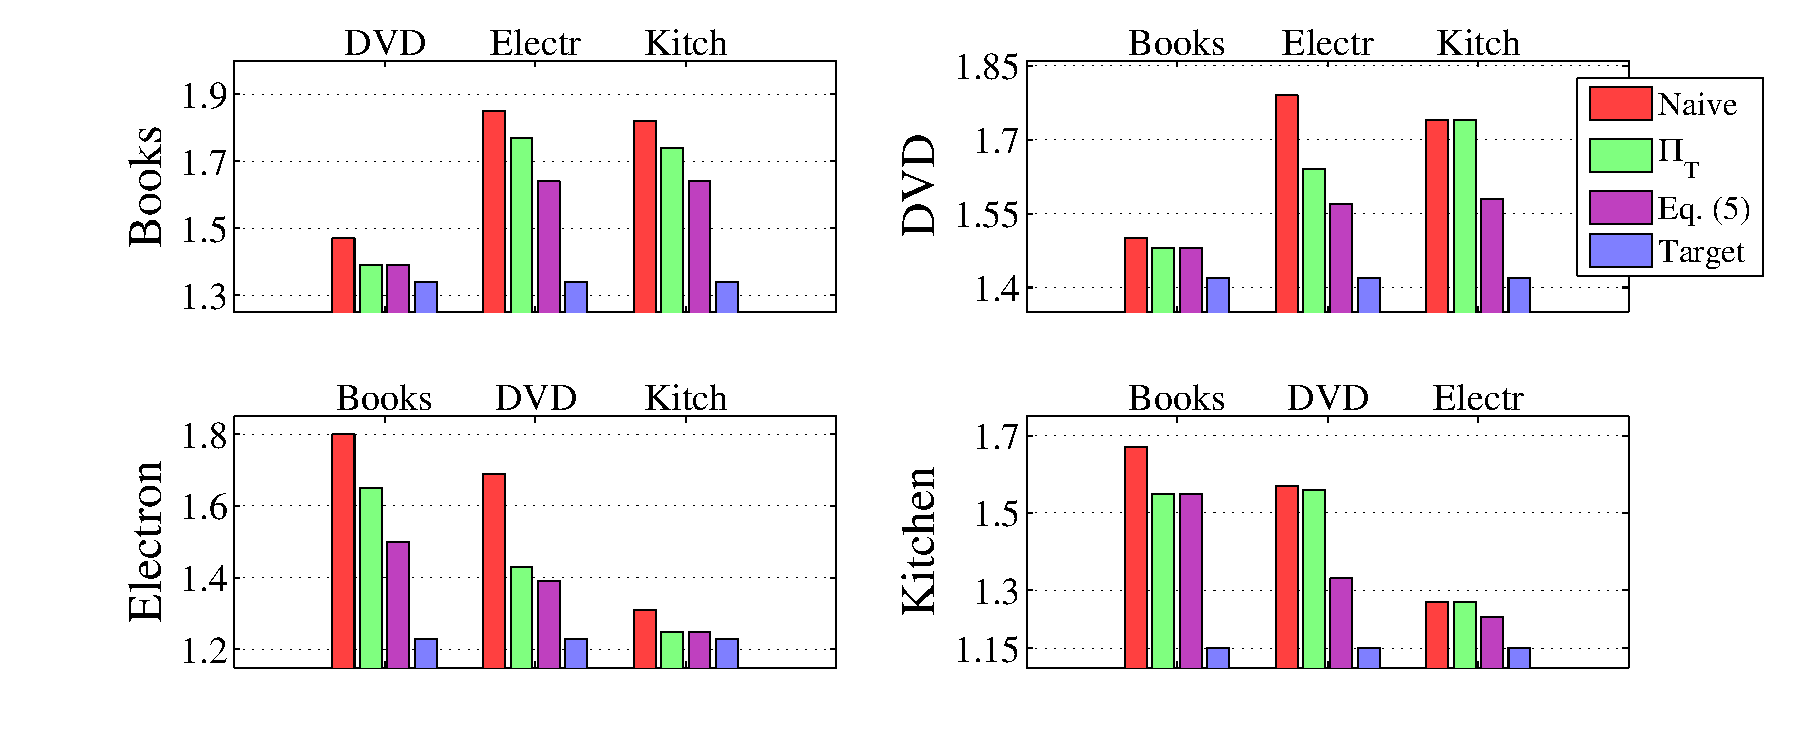
\includegraphics[width=6.4in]{figures/sentiment.pdf}
\vspace{-0.3in}
\caption{Squared error for the sentiment data (1-5 stars).  Each of
  the four graphs shows results for a single target domain, which is
  labeled on the Y-axis.  Clockwise from top left are books, dvds,
  kitchen, and electronics.  Each group of three bars represents one
  pair of domains, and the error bars indicate the standard deviation
  over 10 random draws of source training and target test set.  The
  red bar is the na\"{i}ve algorithm which does not exploit $\Projt$
  or $\Projs$.  The green is our coupled learning algorithm with only
  source data.  The blue (train on target) bars are unaffected by
  source and constant across target domains.}
\label{fig:sentiment_results}
\end{figure}

We begin by evaluating the target performance of our coupled learning
algorithm when learning only from labeled source data.
Figure~\ref{fig:sentiment_results} shows the performance on sentiment
data of the coupled model (in green) versus a na\"{i}ve model (in red)
which simply learns based on the original feature representation,
without taking advantage of projections $\Projt$ and $\Projs$.  The
blue bars train a model directly on the target data and can be thought
of as a ``lower bound'' on error for adaptation.  We defer comparisons
with other adaptation algorithms to Section~\ref{subsec:other}.

\begin{wrapfigure}{l}{3.5in}
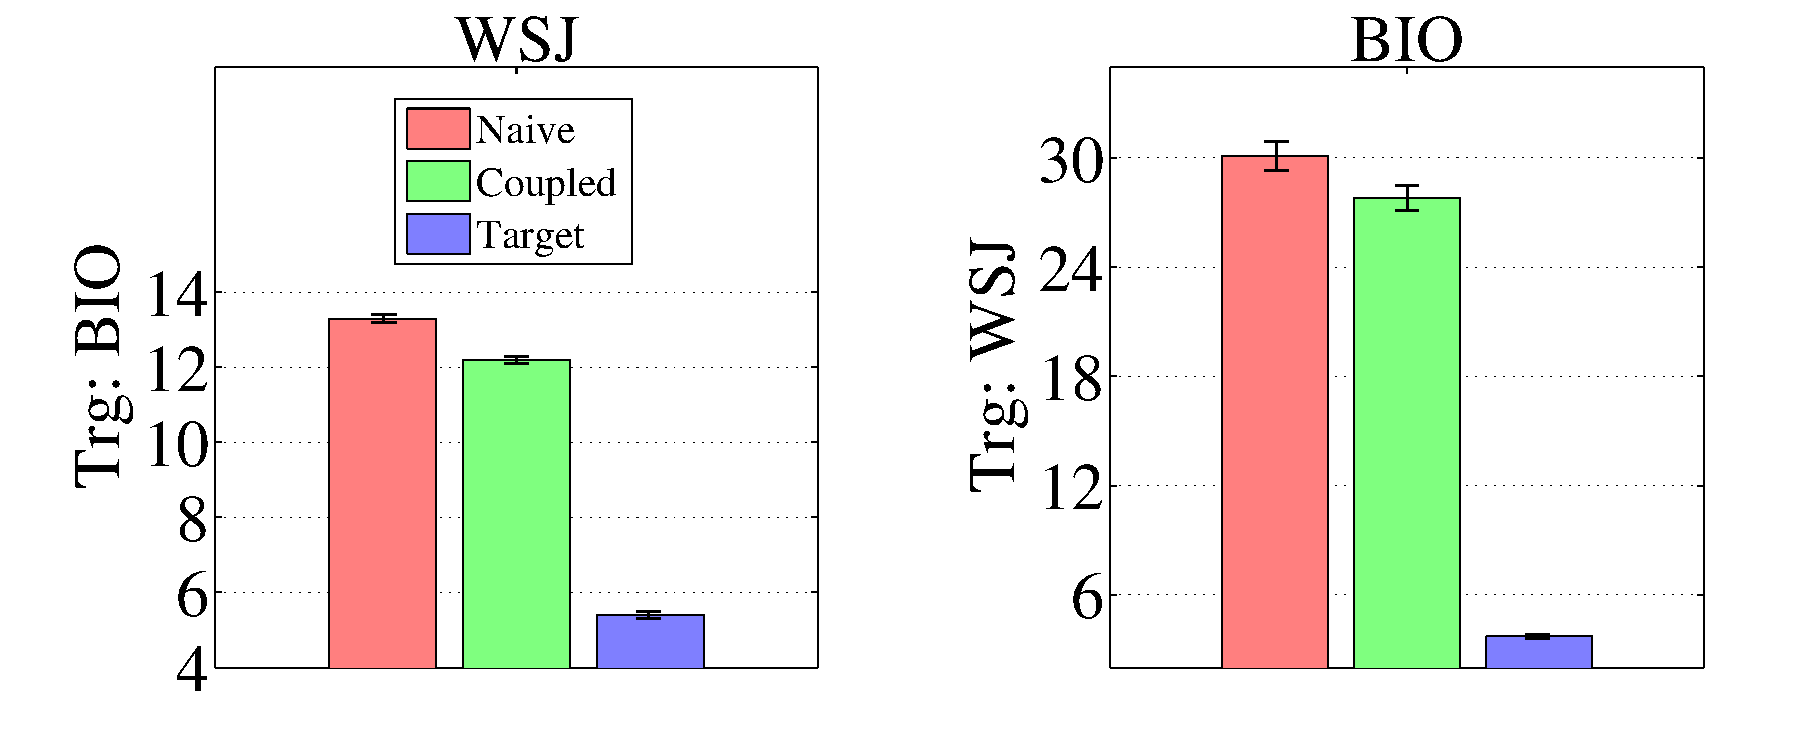
\includegraphics[width=3.5in]{figures/pos.pdf}
\caption{Per-token error for the part of speech tagging task.  Left is from WSJ to BIO.  Right is from BIO to WSJ.  The algorithms are the same as in Figure~\ref{fig:sentiment_results}.}
\label{fig:pos_results}
\end{wrapfigure}

Since we are able to incorporate unseen features via the shared
representation, our theory predicts an improvement in target
performance.  Our algorithm never causes an increase in error and
often greatly improves improves over the na\"{i}ve model.  It is also
worth mentioning that certain pairs of domains overlap less than
others.  For example, books and DVDs are highly overlapping in
vocabulary usage, but books and kitchen appliances are not.  Our
method performs especially well (relative to the baseline) for those
pairs of very dissimilar domains where there are many new,
target-specific features.  We explore this further in
Section~\ref{sec:newnorm}

Figure~\ref{fig:pos_results} illustrates the the coupled learner for
part of speech tagging.  In this case, the variance among experiments
is much smaller due to the larger training data.  Once again, our
method always improves over the na\"{i}ve model.  Finally, we note
that because of data asymmetry, our WSJ models are generally much
better than our BIO models.  In particular, in the right-hand plot,
the BIO source model is trained on only 12,500 words, but the WSJ
target model is trained on 1 million.

\subsection{Adaptation with Source and Target}

\begin{figure}
\hspace{-0.5in}
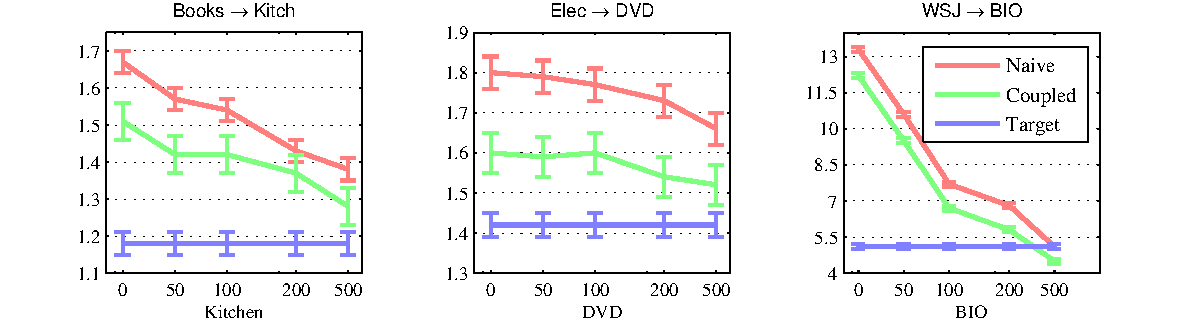
\includegraphics[width=6.5in]{figures/withtarget.pdf}
\caption{Including some target data.  Each figure represents one pair of domains.  The $x$ axis indicates the amount of target data.}
\label{fig:withtarget}
\end{figure}

Our theory indicates that target data can be helpful in stabilizing
predictors learned from the source domain, especially when the domains
diverge somewhat on the shared subspace.  Of course, we also expect
target data to help the na\"{i}ve algorithm as well, but here we show
that our coupled predictors continue to consistently improve over the
naive predictors, even when we do have labeled target training data.
Figure~\ref{fig:withtarget} demonstrates this for three selected
domain pairs.  In the case of part of speech tagging, we use all of
the available target labeled data, and in this case we see a
significant improvement over the target only model (blue curve).
Because of space constraints, we don't show results for all pairs of
domains, but these results are representative.

\subsection{Use of target-specific features}
\label{sec:newnorm}

\begin{figure}
\begin{center}
\begin{tabular}{|c|c|c|}
\hline
\vspace{-0.14in}\\
Adaptation & Negative Target Features & Positive Target Features \\
\hline
\vspace{-0.14in}\\
Books to Kitch & \emph{mush, bad quality, broke,} & \emph{dishwasher, evenly, super easy} \\ 
& \emph{warranty, coffeemaker} & \emph{works great, great product}\\
\hline
\vspace{-0.14in}\\
Kitch to Books & \emph{critique, trite, religious} & \emph{wonderful book, introduction to} \\
& \emph{the publisher, the author} & \emph{illustrations, good reference, relationships} \\
\hline
\end{tabular}
\end{center}
\label{fig:target-specific}
\caption{Illustration of how the coupled learner
  (Equation~\ref{eq:coupled}) uses unique target-specific features for the
  pair of sentiment domains \emph{Books} and \emph{Kitchen}.  We train
  a model using only source data and then find the most positive and
  negative features that are target specific by examining the weights
  under $\left[w_{t}\Projt\right]_{t,\perp}$.}
\end{figure}

Here we briefly explore how the coupled learner puts weight on unseen
features.  One simple test is to measure the relative mass of the
weight vector that is devoted to target-specific features under
different models.  Under the na\"{i}ve model, this is 0.  Under the
shared representation, it is the proportion of $w_{t}\Projt$ devoted
to genuinely unique features.  That is, $\frac{||\left[w_{t}\Projt\right]_{t,\perp}||^{2}_{2}}{||w_{t} \Projt||^{2}_{2}}$.  This quantity
is on average 9.5\% across all sentiment adaptation task pairs and
32\% for part of speech tag adaptation.  A more qualitative way to
observe the use of target specific features is shown in figure
\ref{fig:target-specific}.  Here we selected the top target-specific
words (never observed in the source) that received high weight under
$w_{t}\Projt$.  Intuitively, the ability to assign high weight to
words like \emph{illustrations} when training on only kitchen
appliances can help us generalize better.

\subsection{Validity of Assumptions}

While our theory depends on Assumptions~\ref{ass:same_task} and
\ref{ass:dim_red}, we do not expect them to hold exactly in practice.
Here we examine the extent to which they hold true for our particular
tasks.  The basic idea is to exploit the fact that we do possess
labeled target data for the two data sets to examine source and target
performance under different conditions.  For
Assumption~\ref{ass:same_task}, we compare the performance of a joint
predictor with the performance of a predictor trained on just one
domain.  If these two differ by a small amount, then
Assumption~\ref{ass:same_task} approximately holds.  Training a joint
predictor on books and kitchen appliance reviews together results in a
1.38 mean squared error on books, versus 1.35 if we train a predictor
from books alone.  On kitchen appliances, the joint error is 1.23
versus 1.19 for the individual predictor.  For part-of-speech tagging,
the results are similar: 4.2 joint error versus 3.7 WSJ-only error on
the Wall Street Journal.

For Assumption~\ref{ass:dim_red}, we performed a similar set of
experiments, training with both the reduced-dimensionality
representation (under $\Projd$) and the full feature representation
with all the in-domain training data we had.  For the WSJ, the reduced
dimensional representation achieves 4.2\% error (versus 3.7\% with the
original feature representation).  For DVDs, the reduced-dimensional
representation achieves a 1.47 mean squared error versus a 1.41 mean
squared error for electronics.  For electronics, the
reduced-dimensional representation achieves a 1.23 mean squared error
versus a 1.21 for the full representation.

\subsection{Alternative Adaptation Algorithms}
\label{subsec:other}

Our coupled learning approach performs well for domain adaptation, but
it is not the only algorithm designed for this problems.  Of the
empirical algorithms, the structural correspondence learning work of
Blitzer et al.~\cite{blitzer06} is the most closely-related, but we
note that on the same sentiment data set that algorithm did not give
as consistent gains as ours (and indeed sometimes hurt performance).
The instance weighting algorithms advocated for sample selection bias
correction~\cite{huang07,cortes08} are designed for cases when the
distributions share support and are thus not appropriate for our
setting, but we do note that Jiang and Zhai~\cite{jiang07} report poor
performance using instance weighting for the PoS tagging task.  

When labeled data does exist, there do exist other algorithms that
exploit it by specifically seeking to relax
Assumption~\ref{ass:same_task}~\cite{argyriou07,daume07,finkel09}.
These algorithms do not exploit unlabeled target data, however, and
thus are not directly comparable to our coupled learner.  Indeed, they
are complementary and could potentially give gains when used together
with our coupled representation, although exploration of that is
beyond the scope of this paper.
